% **** Szablon pracy magisterskiej, licencjackiej lub inżynierskiej ****

\documentclass[polish,12pt,twoside,a4paper]{report}

% *************** Definicje stylu dokumentu ***************

% *********************************************************************************
% W pliku tym zdefiniowany jest wygl¹d dokumentu.
% Zmiany tutaj nie s¹ konieczne o ile nie zamierzasz zmieniaæ wygl¹du dokumentu.
% *********************************************************************************

% *************** Za³adowanie pakietów ***************
\usepackage[a4paper,twoside,left=2.0cm,right=1.5cm,top=1.5cm,bottom=1.5cm]{geometry}
\usepackage[T1]{fontenc}
%\usepackage[cp1250]{inputenc}
\usepackage[utf8]{inputenc}
\usepackage[polish]{babel}
\usepackage{amsmath}
\usepackage{amsfonts}
\usepackage{graphicx}
\usepackage{graphics}
\usepackage{times}
\usepackage{indentfirst}%wciecia a nowych akapitach
\usepackage{listings}
\usepackage{url}
\usepackage[colorlinks=true, linkcolor=black, urlcolor=black, citecolor=black]{hyperref}

\selectlanguage{polish}

%szerokoœœ wciêæ
\setlength{\parindent}{1.25cm}

%numeracja stron
\usepackage{fancyhdr}
\pagestyle{fancy}
\fancyhf{} % usun biezace ustawienia pagin
\fancyhead[LE,RO]{ }
\fancyhead[LO]{ }
\fancyhead[RE]{ }
\fancyfoot[LE,RO]{\small\thepage}
\fancyfoot[LO]{ }
\fancyfoot[RE]{ }
\renewcommand{\headrulewidth}{0.0pt}
\renewcommand{\footrulewidth}{0.0pt}
\addtolength{\headheight}{0.0pt} % pionowy odstep na kreske
\fancypagestyle{plain}{%
\fancyhead{} % usun p. górne na stronach pozbawionych
% numeracji (plain)
\renewcommand{\headrulewidth}{0.0pt} % pozioma kreska
}

% *************** Definicje niektórych kolorów ***************
\usepackage{color}

\definecolor{greenyellow}   {cmyk}{0.15, 0   , 0.69, 0   }
\definecolor{yellow}        {cmyk}{0   , 0   , 1   , 0   }
\definecolor{goldenrod}     {cmyk}{0   , 0.10, 0.84, 0   }
\definecolor{dandelion}     {cmyk}{0   , 0.29, 0.84, 0   }
\definecolor{apricot}       {cmyk}{0   , 0.32, 0.52, 0   }
\definecolor{peach}         {cmyk}{0   , 0.50, 0.70, 0   }
\definecolor{melon}         {cmyk}{0   , 0.46, 0.50, 0   }
\definecolor{yelloworange}  {cmyk}{0   , 0.42, 1   , 0   }
\definecolor{orange}        {cmyk}{0   , 0.61, 0.87, 0   }
\definecolor{burntorange}   {cmyk}{0   , 0.51, 1   , 0   }
\definecolor{bittersweet}   {cmyk}{0   , 0.75, 1   , 0.24}
\definecolor{redorange}     {cmyk}{0   , 0.77, 0.87, 0   }
\definecolor{mahogany}      {cmyk}{0   , 0.85, 0.87, 0.35}
\definecolor{maroon}        {cmyk}{0   , 0.87, 0.68, 0.32}
\definecolor{brickred}      {cmyk}{0   , 0.89, 0.94, 0.28}
\definecolor{red}           {cmyk}{0   , 1   , 1   , 0   }
\definecolor{orangered}     {cmyk}{0   , 1   , 0.50, 0   }
\definecolor{rubinered}     {cmyk}{0   , 1   , 0.13, 0   }
\definecolor{wildstrawberry}{cmyk}{0   , 0.96, 0.39, 0   }
\definecolor{salmon}        {cmyk}{0   , 0.53, 0.38, 0   }
\definecolor{carnationpink} {cmyk}{0   , 0.63, 0   , 0   }
\definecolor{magenta}       {cmyk}{0   , 1   , 0   , 0   }
\definecolor{violetred}     {cmyk}{0   , 0.81, 0   , 0   }
\definecolor{rhodamine}     {cmyk}{0   , 0.82, 0   , 0   }
\definecolor{mulberry}      {cmyk}{0.34, 0.90, 0   , 0.02}
\definecolor{redviolet}     {cmyk}{0.07, 0.90, 0   , 0.34}
\definecolor{fuchsia}       {cmyk}{0.47, 0.91, 0   , 0.08}
\definecolor{lavender}      {cmyk}{0   , 0.48, 0   , 0   }
\definecolor{thistle}       {cmyk}{0.12, 0.59, 0   , 0   }
\definecolor{orchid}        {cmyk}{0.32, 0.64, 0   , 0   }
\definecolor{darkorchid}    {cmyk}{0.40, 0.80, 0.20, 0   }
\definecolor{purple}        {cmyk}{0.45, 0.86, 0   , 0   }
\definecolor{plum}          {cmyk}{0.50, 1   , 0   , 0   }
\definecolor{violet}        {cmyk}{0.79, 0.88, 0   , 0   }
\definecolor{royalpurple}   {cmyk}{0.75, 0.90, 0   , 0   }
\definecolor{blueviolet}    {cmyk}{0.86, 0.91, 0   , 0.04}
\definecolor{periwinkle}    {cmyk}{0.57, 0.55, 0   , 0   }
\definecolor{cadetblue}     {cmyk}{0.62, 0.57, 0.23, 0   }
\definecolor{cornflowerblue}{cmyk}{0.65, 0.13, 0   , 0   }
\definecolor{midnightblue}  {cmyk}{0.98, 0.13, 0   , 0.43}
\definecolor{navyblue}      {cmyk}{0.94, 0.54, 0   , 0   }
\definecolor{royalblue}     {cmyk}{1   , 0.50, 0   , 0   }
\definecolor{blue}          {cmyk}{1   , 1   , 0   , 0   }
\definecolor{cerulean}      {cmyk}{0.94, 0.11, 0   , 0   }
\definecolor{cyan}          {cmyk}{1   , 0   , 0   , 0   }
\definecolor{processblue}   {cmyk}{0.96, 0   , 0   , 0   }
\definecolor{skyblue}       {cmyk}{0.62, 0   , 0.12, 0   }
\definecolor{turquoise}     {cmyk}{0.85, 0   , 0.20, 0   }
\definecolor{tealblue}      {cmyk}{0.86, 0   , 0.34, 0.02}
\definecolor{aquamarine}    {cmyk}{0.82, 0   , 0.30, 0   }
\definecolor{bluegreen}     {cmyk}{0.85, 0   , 0.33, 0   }
\definecolor{emerald}       {cmyk}{1   , 0   , 0.50, 0   }
\definecolor{junglegreen}   {cmyk}{0.99, 0   , 0.52, 0   }
\definecolor{seagreen}      {cmyk}{0.69, 0   , 0.50, 0   }
\definecolor{green}         {cmyk}{1   , 0   , 1   , 0   }
\definecolor{forestgreen}   {cmyk}{0.91, 0   , 0.88, 0.12}
\definecolor{pinegreen}     {cmyk}{0.92, 0   , 0.59, 0.25}
\definecolor{limegreen}     {cmyk}{0.50, 0   , 1   , 0   }
\definecolor{yellowgreen}   {cmyk}{0.44, 0   , 0.74, 0   }
\definecolor{springgreen}   {cmyk}{0.26, 0   , 0.76, 0   }
\definecolor{olivegreen}    {cmyk}{0.64, 0   , 0.95, 0.40}
\definecolor{rawsienna}     {cmyk}{0   , 0.72, 1   , 0.45}
\definecolor{sepia}         {cmyk}{0   , 0.83, 1   , 0.70}
\definecolor{brown}         {cmyk}{0   , 0.81, 1   , 0.60}
\definecolor{tan}           {cmyk}{0.14, 0.42, 0.56, 0   }
\definecolor{gray}          {cmyk}{0   , 0   , 0   , 0.50}
\definecolor{black}         {cmyk}{0   , 0   , 0   , 1   }
\definecolor{white}         {cmyk}{0   , 0   , 0   , 0   } 

% *************** Koniec definicji stylu dokumentu ***************


%definicja przydatnych poleceń
\newcommand{\wydzial}{KOLEGIUM INFORMATYKI STOSOWANEJ}
\newcommand{\kierunek}{Kierunek: INFORMATYKA}
\newcommand{\specjalnosc}{Specjalność: {Inżynieria Danych (ID)}}
\newcommand{\autor}{Karol Grabowski}
\newcommand{\album}{Nr albumu w69781}
\newcommand{\temat}{System biura podróży}
\newcommand{\promotor}{mgr inż. Ewa Żesławska}
\newcommand{\typpracy}{Praca projektowa programowanie obiektowe C\#}
\newcommand{\miasto}{Rzeszów}
\newcommand{\rok}{2025}

\begin{document}

% *************** Włączenie definicji pierwszych stron ***************
% *************** Strony tytułowe ***************

% ************************************************************
% W tym miejscu znajduje sie definicja wyglądu pierwszych stron:
% strony tytułowej, strony z oświadczeniem o treści pracy
% i strony ze spisem treści
% ************************************************************
% *************** Strona tytułowa ***************
%umieszczenie logo i nazwy uczelni
\noindent
\parbox{65mm}{
\includegraphics[width=13.0cm, height=3.0cm]{logoWSIiZ}}

\vspace{10mm}
\begin{center}
{\Large{}\textbf{\wydzial}}
\end{center}
\vspace{10mm}
\noindent
\hspace{30mm}{\Large{}\textbf{\kierunek}}\\

\noindent
\hspace{30mm}{\Large{}\textbf{\specjalnosc}}
\vspace{30mm}
\begin{center}
	{\large{}\autor}\\
	{\large{}\album}\\
	\vspace{15pt}
	{\huge{}\textbf{\textit{\temat}}}\\
	\vspace{20pt}
	{\normalsize{}Prowadzący: \promotor}\\
	\vspace{100pt}
	{\LARGE{}\textbf{\typpracy}}\\
	\vspace{190pt}
	{\large{}\textbf{\miasto {} \rok}}
\end{center}

% pusta zawartość stopki - brak numeru strony
\thispagestyle{empty}

% *************** Strona z oświadczeniem o treści pracy ***************
\newpage
\text{}

\thispagestyle{empty}
\newpage


% *************** Spis treści ***************
\tableofcontents
% pusta zawartość stopki - brak numeru strony
\thispagestyle{empty}
\newpage

% *************** Koniec pliku front.tex ***************



% *************** Część główna pracy ***************
\chapter*{Wstęp}

Współczesny rynek turystyczny charakteryzuje się nieustanną dynamiką, a klienci oczekują coraz bardziej zróżnicowanych i dostosowanych do ich potrzeb usług. W związku z tym biura podróży muszą wykorzystywać nowoczesne technologie, które pozwolą im utrzymać konkurencyjność i spełniać wymagania rynku. Wspomaganie codziennej działalności biura podróży za pomocą systemów informatycznych staje się kluczowe w procesach zarządzania ofertami, rezerwacjami, a także w obiegu informacji dotyczących płatności i rozliczeń. Tradycyjne, papierowe metody obsługi mogą prowadzić do błędów, opóźnień i utrudnionego dostępu do danych, co negatywnie wpływa na efektywność pracy oraz satysfakcję klientów. W odpowiedzi na te problemy, niniejszy projekt ma na celu stworzenie systemu informatycznego, który będzie kompleksowo wspierać zarządzanie biurem podróży.

System ten pozwoli na łatwe tworzenie, edytowanie oraz usuwanie ofert turystycznych, umożliwiając szybką reakcję na zmieniające się potrzeby rynku oraz na wprowadzanie nowych produktów do oferty. Dodatkowo, aplikacja będzie umożliwiać dokonywanie rezerwacji biletów na dostępne oferty, co zapewni wygodę klientom oraz pozwoli na pełną kontrolę nad rezerwacjami dla pracowników biura. Ważnym aspektem systemu będzie również moduł umożliwiający obsługę rozliczeń finansowych, który zautomatyzuje procesy związane z płatnościami za usługi oraz umożliwi szybkie i przejrzyste rozliczanie się z klientami.

Projekt zostanie opracowany w języku C\#, co pozwoli na stworzenie wydajnej, bezpiecznej i skalowalnej aplikacji. Wykorzystanie tego języka umożliwia budowę systemu, który będzie łatwy do rozbudowy, dostosowania oraz utrzymania w przyszłości, co stanowi istotny element w kontekście rozwijających się potrzeb biura podróży. Projektowana aplikacja będzie zawierała intuicyjny interfejs użytkownika, który ułatwi pracownikom biura szybkie wykonywanie niezbędnych operacji oraz pozwoli klientom na komfortowe korzystanie z dostępnych usług.


\addcontentsline{toc}{chapter}{Wstęp}
\newpage
% ********** Rozdział 1 **********
\chapter{Opis założeń projektu}
\section{Cele projetu}
%\subsection{Tytuł pierwszego podpunktu}

Celem niniejszego projektu jest opracowanie zaawansowanego systemu informatycznego, którego głównym zadaniem będzie wsparcie procesów związanych z zarządzaniem ofertami turystycznymi, rezerwacjami oraz rozliczeniami w biurze podróży. Projekt zakłada stworzenie elastycznego narzędzia umożliwiającego bieżącą modyfikację i aktualizację oferty turystycznej poprzez funkcjonalności pozwalające na tworzenie, edytowanie oraz usuwanie poszczególnych pozycji oferty, co umożliwi dynamiczne dostosowywanie się do zmieniających się warunków rynkowych.
System zostanie wyposażony w moduł rezerwacyjny, który umożliwi klientom samodzielne dokonywanie rezerwacji biletów, a jednocześnie pozwoli pracownikom biura na efektywne zarządzanie procesem rezerwacyjnym. Wdrożenie funkcjonalności rozliczeniowych stanowi kolejny kluczowy element projektu, który ma na celu usprawnienie kontroli płatności oraz rozliczeń finansowych, co przyczyni się do zwiększenia przejrzystości oraz efektywności zarządzania finansami w biurze podróży.


\section{Wymagania funkcjonale i niefunkcjonalne}

\noindent \textbf{Wymagania funkcjonalne}
\begin{itemize}
    \item Zarządzanie ofertami: Użytkownicy systemu (pracownicy biura) mogą dodawać nowe oferty, edytować ich parametry oraz usuwać je z bazy.
    \item Prezentacja oferty: Klienci mają możliwość przeglądania pełnych informacji o dostępnych ofertach, takich jak nazwa, destynacja, cena i liczba dostępnych miejsc.
    \item Rezerwacje: System umożliwia klientom dokonywanie rezerwacji wybranych ofert, zapisując te dane w wewnętrznej bazie.
    \item Modyfikacja rezerwacji: Pracownicy biura mogą wprowadzać zmiany w rezerwacjach lub je anulować.
    \item Obsługa płatności: System rejestruje płatności, generuje proste faktury oraz umożliwia przegląd historii transakcji.
    \item Zarządzanie użytkownikami: Możliwość tworzenia kont, przypisywania im określonych ról oraz ograniczania dostępu do niektórych funkcji systemu.
\end{itemize}

\noindent \textbf{Wymagania niefunkcjonalne }
\begin{itemize}
    \item Wydajność: System powinien działać sprawnie nawet przy dużej liczbie ofert i rezerwacji. 
    \item Skalowalność: Aplikacja musi umożliwiać łatwe dodawanie nowych modułów i funkcjonalności.
    \item Bezpieczeństwo: Dane osobowe klientów i informacje finansowe muszą być odpowiednio chronione, co w przyszłości można rozszerzyć o mechanizmy szyfrowania i autoryzacji.
    \item Przyjazny interfejs: Nawet jeśli obecnie jest to interfejs konsolowy, system powinien być intuicyjny i łatwy w obsłudze.
    \item Kompatybilność: System oparty na technologii .NET musi działać na różnych systemach operacyjnych oraz być zgodny z aktualnymi standardami.
    \item Niezawodność: System powinien minimalizować ryzyko awarii oraz umożliwiać tworzenie kopii zapasowych danych.
\end{itemize}
 


% ********** Koniec rozdziału **********

\newpage
% ********** Rozdział 2 **********
\chapter{Opis struktury projektu}
Projekt został zbudowany w oparciu o modułową architekturę, dzięki której łatwo można zarządzać poszczególnymi częściami systemu. Główne komponenty to:
\begin{figure}[htbp]
  \centering
  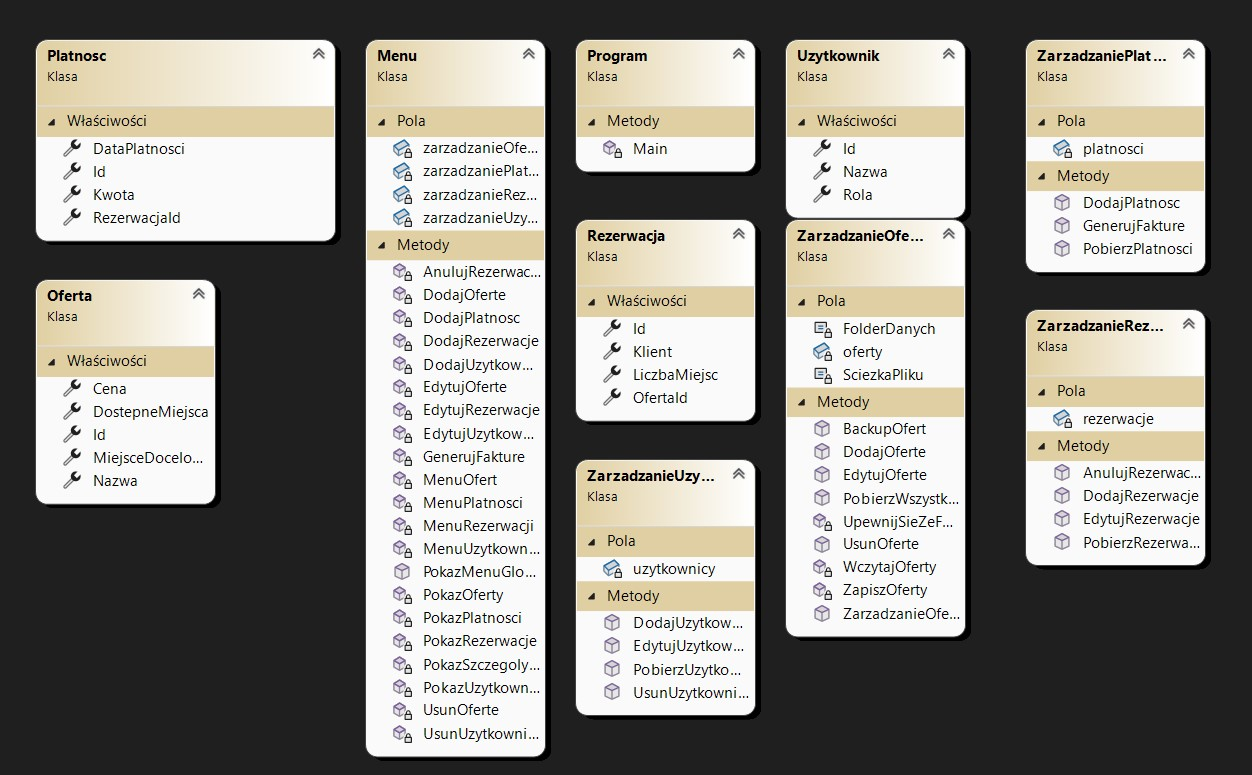
\includegraphics[width=1\textwidth]{figures/diagram_klas.jpg} 
  \caption{Diagram klas użytych w programie.}
  \label{fig:obrazek}
\end{figure}

\noindent \textbf{Modele Danych:}
\begin{itemize}
    \item \textbf{Oferta} – reprezentuje ofertę turystyczną, przechowując dane takie jak nazwa, destynacja, cena i dostępność miejsc.
    \item \textbf{Rezerwacja} – zawiera informacje o rezerwacjach, w tym identyfikator oferty, dane klienta oraz liczbę zarezerwowanych miejsc.
    \item \textbf{Płatność} – przechowuje dane dotyczące płatności, w tym kwotę, datę oraz powiązanie z konkretną rezerwacją.
    \item \textbf{Użytkownik} – model użytkownika systemu, który pozwala na zarządzanie kontami i uprawnieniami.
\end{itemize}
\noindent \textbf{Logika Biznesowa:}
Każdy z modułów zarządzających (oferty, rezerwacje, płatności, użytkownicy) zawiera operacje CRUD, czyli funkcje umożliwiające tworzenie, odczyt, modyfikację i usuwanie danych. Moduły te korzystają z wbudowanych bibliotek .NET, takich jak \texttt{System.IO} i \texttt{System.Text.Json}, do operacji na plikach oraz serializacji danych.

\noindent \textbf{Warstwa Prezentacji:}
Interfejs użytkownika opiera się na prostym menu konsolowym, które umożliwia nawigację między poszczególnymi modułami systemu. Użytkownik może wybrać odpowiednią opcję, aby wykonać operacje związane z zarządzaniem ofertami, rezerwacjami, płatnościami i kontami.

\noindent \textbf{Punkt Wejścia:}
Program rozpoczyna działanie od metody \texttt{Main()}, która inicjuje obiekt odpowiedzialny za wyświetlenie menu głównego.



\section{Modele Danych}
\subsection*{Klasa \textbf{Oferta}}
\begin{itemize}
    \item \textbf{Atrybuty:}
    \begin{itemize}
        \item \texttt{int Id} -- unikalny identyfikator oferty.
        \item \texttt{string Nazwa} -- nazwa oferty (np. "Wakacje w Grecji").
        \item \texttt{string MiejsceDocelowe} -- miejsce docelowe oferty.
        \item \texttt{decimal Cena} -- cena oferty; typ \texttt{decimal} zapewnia dokładność operacji finansowych.
        \item \texttt{int DostepneMiejsca} -- liczba dostępnych miejsc w ofercie.
    \end{itemize}
    \item \textbf{Metody:}  
    Klasa wykorzystuje autogenerowane właściwości (get; set;), pełniąc funkcję przechowywania danych bez dodatkowej logiki.
\end{itemize}

\subsection*{Klasa \textbf{Rezerwacja}}
\begin{itemize}
    \item \textbf{Atrybuty:}
    \begin{itemize}
        \item \texttt{int Id} -- unikalny identyfikator rezerwacji.
        \item \texttt{int OfertaId} -- identyfikator powiązanej oferty.
        \item \texttt{string Klient} -- dane klienta (np. imię i nazwisko) dokonującego rezerwacji.
        \item \texttt{int LiczbaMiejsc} -- liczba miejsc zarezerwowanych przez klienta.
    \end{itemize}
    \item \textbf{Metody:}  
    Podobnie jak w klasie \textbf{Oferta}, właściwości przechowują dane bez dodatkowej logiki.
\end{itemize}

\subsection*{Klasa \textbf{Platnosc}}
\begin{itemize}
    \item \textbf{Atrybuty:}
    \begin{itemize}
        \item \texttt{int Id} -- unikalny identyfikator płatności.
        \item \texttt{int RezerwacjaId} -- identyfikator rezerwacji, do której odnosi się płatność.
        \item \texttt{decimal Kwota} -- kwota płatności.
        \item \texttt{string DataPlatnosci} -- data dokonania płatności (jako ciąg znaków).
    \end{itemize}
    \item \textbf{Metody:}  
    Klasa służy do przechowywania danych dotyczących płatności przy użyciu autogenerowanych właściwości.
\end{itemize}

\subsection*{Klasa \textbf{Uzytkownik}}
\begin{itemize}
    \item \textbf{Atrybuty:}
    \begin{itemize}
        \item \texttt{int Id} -- unikalny identyfikator użytkownika.
        \item \texttt{string Nazwa} -- nazwa lub login użytkownika.
        \item \texttt{string Rola} -- rola przypisana użytkownikowi (np. administrator, pracownik, klient).
    \end{itemize}
    \item \textbf{Metody:}  
    Podstawową funkcją klasy jest przechowywanie informacji o użytkowniku.
\end{itemize}

\section{Klasy Zarządzające (Service/Manager Classes)}
\subsection*{Klasa \textbf{ZarzadzanieOfertami}}
\begin{itemize}
    \item \textbf{Atrybuty:}
    \begin{itemize}
        \item \texttt{const string FolderDanych} -- nazwa folderu (np. "Dane") do przechowywania pliku.
        \item \texttt{const string SciezkaPliku} -- pełna ścieżka do pliku JSON (np. "Dane/oferty.json").
        \item \texttt{List<Oferta> oferty} -- lista ofert wczytanych z pliku.
    \end{itemize}
    \item \textbf{Kluczowe Metody:}
    \begin{itemize}
        \item \texttt{ZarzadzanieOfertami()} -- Konstruktor; sprawdza istnienie folderu (metoda \texttt{UpewnijSieZeFolderIstnieje()}), tworzy plik JSON, jeżeli nie istnieje, oraz wczytuje oferty (metoda \texttt{WczytajOferty()}).
        \item \texttt{UpewnijSieZeFolderIstnieje()} -- Sprawdza, czy folder \texttt{FolderDanych} istnieje; w razie potrzeby tworzy go.
        \item \texttt{WczytajOferty()} -- Odczytuje zawartość pliku JSON, deserializuje dane do listy obiektów \texttt{Oferta} i zwraca tę listę.
        \item \texttt{ZapiszOferty()} -- Serializuje listę ofert do formatu JSON i zapisuje ją w pliku.
        \item \texttt{PobierzWszystkieOferty()} -- Zwraca listę wszystkich ofert.
        \item \texttt{DodajOferte(Oferta oferta)} -- Przed dodaniem nowej oferty przypisuje jej unikalne \texttt{Id} i zapisuje ofertę.
        \item \texttt{EdytujOferte(int id, Oferta nowaOferta)} -- Wyszukuje ofertę po \texttt{Id} i aktualizuje jej dane (Nazwa, MiejsceDocelowe, Cena, DostepneMiejsca), a następnie zapisuje zmiany.
        \item \texttt{UsunOferte(int id)} -- Usuwa ofertę o podanym \texttt{Id} z listy i zapisuje zmiany.
        \item \texttt{BackupOfert()} -- Tworzy kopię zapasową pliku JSON z ofertami.
    \end{itemize}
\end{itemize}

\subsection*{Klasa \textbf{ZarzadzanieRezerwacjami}}
\begin{itemize}
    \item \textbf{Atrybuty:}
    \begin{itemize}
        \item \texttt{List<Rezerwacja> rezerwacje} -- lista rezerwacji przechowywana w pamięci.
    \end{itemize}
    \item \textbf{Kluczowe Metody:}
    \begin{itemize}
        \item \texttt{DodajRezerwacje(Rezerwacja rezerwacja)} -- Dodaje nową rezerwację, przypisując jej unikalne \texttt{Id}.
        \item \texttt{EdytujRezerwacje(int id, Rezerwacja nowaRezerwacja)} -- Wyszukuje rezerwację po \texttt{Id} i aktualizuje jej dane (OfertaId, Klient, LiczbaMiejsc).
        \item \texttt{AnulujRezerwacje(int id)} -- Usuwa rezerwację o określonym \texttt{Id} z listy.
        \item \texttt{PobierzRezerwacje()} -- Zwraca aktualną listę rezerwacji.
    \end{itemize}
\end{itemize}

\subsection*{Klasa \textbf{ZarzadzaniePlatnosciami}}
\begin{itemize}
    \item \textbf{Atrybuty:}
    \begin{itemize}
        \item \texttt{List<Platnosc> platnosci} -- lista płatności.
    \end{itemize}
    \item \textbf{Kluczowe Metody:}
    \begin{itemize}
        \item \texttt{DodajPlatnosc(Platnosc platnosc)} -- Dodaje nową płatność, przypisując jej unikalne \texttt{Id}.
        \item \texttt{PobierzPlatnosci()} -- Zwraca listę wszystkich płatności.
        \item \texttt{GenerujFakture(int platnoscId)} -- Wyszukuje płatność po \texttt{Id} i zwraca sformatowaną fakturę zawierającą dane płatności; w przypadku braku płatności, zwraca komunikat o błędzie.
    \end{itemize}
\end{itemize}

\subsection*{Klasa \textbf{ZarzadzanieUzytkownikami}}
\begin{itemize}
    \item \textbf{Atrybuty:}
    \begin{itemize}
        \item \texttt{List<Uzytkownik> uzytkownicy} -- lista użytkowników.
    \end{itemize}
    \item \textbf{Kluczowe Metody:}
    \begin{itemize}
        \item \texttt{DodajUzytkownika(Uzytkownik uzytkownik)} -- Dodaje nowego użytkownika, nadając mu unikalne \texttt{Id}.
        \item \texttt{EdytujUzytkownika(int id, Uzytkownik nowyUzytkownik)} -- Znajduje użytkownika o danym \texttt{Id} i aktualizuje jego dane (Nazwa, Rola).
        \item \texttt{UsunUzytkownika(int id)} -- Usuwa użytkownika o podanym \texttt{Id} z listy.
        \item \texttt{PobierzUzytkownikow()} -- Zwraca listę wszystkich użytkowników.
    \end{itemize}
\end{itemize}

\section{Warstwa Interfejsu Użytkownika}
\subsection*{Klasa \textbf{Menu}}
\begin{itemize}
    \item \textbf{Atrybuty:}
    \begin{itemize}
        \item \texttt{ZarzadzanieOfertami zarzadzanieOfertami} -- obiekt do zarządzania ofertami.
        \item \texttt{ZarzadzanieRezerwacjami zarzadzanieRezerwacjami} -- obiekt do zarządzania rezerwacjami.
        \item \texttt{ZarzadzaniePlatnosciami zarzadzaniePlatnosciami} -- obiekt do obsługi płatności.
        \item \texttt{ZarzadzanieUzytkownikami zarzadzanieUzytkownikami} -- obiekt do zarządzania użytkownikami.
    \end{itemize}
    \item \textbf{Kluczowe Metody:}
    \begin{itemize}
        \item \texttt{PokazMenuGlowne()} -- Uruchamia główną pętlę interakcji, wyświetlając menu główne i kierując użytkownika do odpowiednich podmenu.
        \item \textbf{Podmenu ofert:}
        \begin{itemize}
            \item \texttt{MenuOfert()} -- Wyświetla opcje zarządzania ofertami.
            \item \texttt{PokazOferty()} -- Prezentuje listę wszystkich ofert.
            \item \texttt{PokazSzczegolyOferty()} -- Po podaniu ID, wyświetla szczegóły wybranej oferty.
            \item \texttt{DodajOferte()} -- Pobiera dane od użytkownika, tworzy nową ofertę i wywołuje metodę dodawania w module ofert.
            \item \texttt{EdytujOferte()} -- Umożliwia edycję istniejącej oferty.
            \item \texttt{UsunOferte()} -- Umożliwia usunięcie oferty.
        \end{itemize}
        \item \textbf{Podmenu rezerwacji:}
        \begin{itemize}
            \item \texttt{MenuRezerwacji()} -- Wyświetla opcje związane z rezerwacjami.
            \item \texttt{DodajRezerwacje()} -- Pobiera dane wejściowe i dodaje nową rezerwację.
            \item \texttt{EdytujRezerwacje()} -- Umożliwia edycję wybranej rezerwacji.
            \item \texttt{AnulujRezerwacje()} -- Pozwala na anulowanie rezerwacji.
            \item \texttt{PokazRezerwacje()} -- Wyświetla listę rezerwacji.
        \end{itemize}
        \item \textbf{Podmenu płatności:}
        \begin{itemize}
            \item \texttt{MenuPlatnosci()} -- Wyświetla opcje związane z płatnościami.
            \item \texttt{DodajPlatnosc()} -- Dodaje nową płatność na podstawie danych wejściowych.
            \item \texttt{PokazPlatnosci()} -- Prezentuje listę płatności.
            \item \texttt{GenerujFakture()} -- Generuje i wyświetla fakturę dla wybranej płatności.
        \end{itemize}
        \item \textbf{Podmenu użytkowników:}
        \begin{itemize}
            \item \texttt{MenuUzytkownikow()} -- Wyświetla opcje zarządzania użytkownikami.
            \item \texttt{DodajUzytkownika()} -- Dodaje nowego użytkownika.
            \item \texttt{EdytujUzytkownika()} -- Umożliwia edycję danych użytkownika.
            \item \texttt{UsunUzytkownika()} -- Pozwala na usunięcie użytkownika.
            \item \texttt{PokazUzytkownikow()} -- Wyświetla listę użytkowników.
        \end{itemize}
    \end{itemize}
\end{itemize}

\section{Klasa Główna}
\subsection*{Klasa \textbf{Program}}
\begin{itemize}
    \item \textbf{Metody:}
    \begin{itemize}
        \item \texttt{Main()} -- Główna metoda wejścia do aplikacji. Tworzy instancję klasy \textbf{Menu} i wywołuje metodę \texttt{PokazMenuGlowne()}, inicjując interakcję z użytkownikiem.
    \end{itemize}
\end{itemize}

Hierarchia klas w systemie zarządzania biurem podróży została zaprojektowana w sposób modularny, co umożliwia oddzielenie modelu danych (Oferta, Rezerwacja, Platnosc, Uzytkownik) od logiki biznesowej (moduły ZarzadzanieOfertami, ZarzadzanieRezerwacjami, ZarzadzaniePlatnosciami, ZarzadzanieUzytkownikami) oraz interfejsu użytkownika (klasa Menu). Kluczowe metody umożliwiają wykonywanie operacji CRUD na danych oraz zapewniają prostą obsługę aplikacji przez użytkownika. Główny punkt wejścia, metoda Main() w klasie Program, inicjuje cały proces, uruchamiając główne menu i umożliwiając interakcję z systemem.

% ********** Koniec rozdziału **********

\newpage
% ********** Rozdział 4 **********
\chapter{Harmonogram realizacji projektu}
\section{Harmonogram realizacji projektu}
W tym rozdziale przedstawiono harmonogram projektu w formie diagramu Gantta. Jego celem jest graficzne zobrazowanie planu, etapów projektu oraz wzajemnych zależności czasowych między poszczególnymi zadaniami.

\subsection{Opis Diagramu Gantta}
Diagram Gantta prezentuje szczegółowy harmonogram realizacji projektu, w ramach którego wyróżniono następujące etapy:\\
\noindent\textbf{Tworzenie założeń projektu:} Przeprowadzenie analizy wymagań, sporządzenie dokumentacji oraz opracowanie planu realizacji.\\[1ex]
\noindent\textbf{Kodowanie:} Implementacja i integracja poszczególnych modułów aplikacji.\\[1ex]
\noindent\textbf{Tworzenie dokumentacji:} Opracowanie kompletnej dokumentacji technicznej oraz użytkowej.\\[1ex]
\noindent\textbf{Obrona projektu:} Przygotowanie prezentacji oraz obrona projektu przed komisją.


\begin{figure}[htbp]
  \centering
  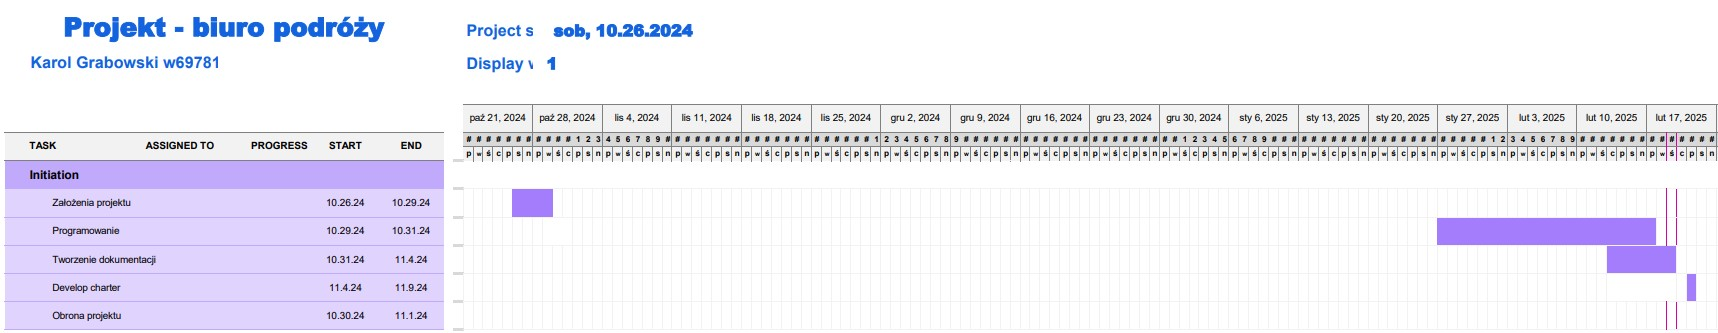
\includegraphics[width=1.1\textwidth]{figures/diagram_gannta.jpg} 
  \caption{Diagram Gantta przedstawiający harmonogram realizacji projektu}
  \label{fig:obrazek}
\end{figure}
\subsection{Napotkane problemy i trudności podczas realizacji projektu}
Podczas tworzenia systemu zarządzania biurem podróży napotkałem na kilka kluczowych wyzwań. Pierwszym z nich było ustalenie odpowiedniej architektury systemu. Zależało mi na tym, aby był on modułowy i skalowalny, co oznaczało łatwość w dodawaniu nowych funkcjonalności. W praktyce wymagało to oddzielenia modelu danych od logiki biznesowej oraz interfejsu użytkownika. Trudnością okazało się zaprojektowanie spójnego interfejsu komunikacyjnego między modułami, aby operacje związane z ofertami, rezerwacjami i płatnościami były zintegrowane i działały harmonijnie.

Kolejnym wyzwaniem było zarządzanie danymi. Przypisanie unikalnych identyfikatorów do ofert, rezerwacji, płatności i użytkowników stanowiło problem, zwłaszcza na początku projektu. Zastosowanie funkcji takich jak „Any()” czy „Max()” w LINQ ułatwiło generowanie tych identyfikatorów, ale wymagało to starannego dopracowania logiki, aby uniknąć konfliktów i duplikacji. Dodatkowo, wdrożenie zapisu i odczytu danych w formacie JSON wymagało precyzyjnego typowania, szczególnie w przypadku wartości pieniężnych, gdzie użycie typu „decimal” było kluczowe dla zachowania dokładności. Na początku napotykano trudności związane z doborem odpowiednich opcji serializacji, co mogło prowadzić do utraty precyzji danych.

Obsługa plików oraz mechanizmy backupu stanowiły kolejny obszar wyzwań. System musiał regularnie zapisywać dane do pliku JSON oraz tworzyć kopie zapasowe, aby chronić informacje przed utratą. Problemy pojawiały się przy implementacji mechanizmu backupu – kluczowe było uwzględnienie sytuacji, w których plik docelowy już istniał, lub gdy występowały trudności z dostępem do dysku. W miarę postępu projektu optymalizacja operacji na plikach może stać się istotnym wyzwaniem, zwłaszcza przy większej liczbie rekordów, co może prowadzić do wąskich gardeł podczas zapisu i odczytu. Potencjalne rozwiązania obejmują wdrożenie mechanizmów buforowania lub migrację do bardziej zaawansowanej bazy danych.

Nie mniej ważnym aspektem była walidacja danych oraz zapewnienie intuicyjnego interfejsu użytkownika. Konieczne stało się wdrożenie mechanizmów sprawdzania poprawności danych wprowadzanych przez użytkowników, na przykład weryfikacja formatu cen czy dostępności miejsc. Początkowo pojawiały się błędy związane z nieprawidłowymi danymi, co wymagało dodatkowych korekt. Mimo że interfejs został zaprojektowany jako konsolowy, musiał być przejrzysty i czytelny, co nie zawsze było łatwe do osiągnięcia na etapie projektowania.

\section{Informacje o repozytorium}

Zarządzanie projektem odbywało się za pomocą systemu kontroli wersji Git, co pozwoliło na precyzyjne monitorowanie postępów. Ponadto, projekt był hostowany na platformie GitHub, zapewniającej łatwy dostęp do repozytorium oraz narzędzi wspierających współpracę i integrację z innymi systemami. Repozytorium można znaleźć pod adresem:\\

\url{https://github.com/grabowskikarol/w69781_Programowanie_Obiektowe/tree/main/Projekt_w69781/Biuro_podrozy}


% ********** Koniec rozdziału **********
\newpage
% ********** Rozdział 4 **********
\chapter{Prezentacja warstwy użytkowej projektu}
\subsection{Główne Menu Systemu}
Po uruchomieniu aplikacji, użytkownik natychmiast widzi główne menu, które jest punktem wyjścia do wszystkich funkcji systemu. Menu to prezentuje kilka opcji, takich jak:
\begin{itemize}
    \item Zarządzanie ofertami,
    \item Zarządzanie rezerwacjami,
    \item Zarządzanie płatnościami,
    \item Zarządzanie użytkownikami,
    \item Wyjście z aplikacji.
\end{itemize}

\begin{figure}[htbp]
  \centering
  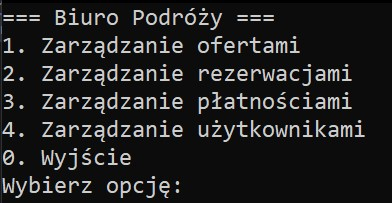
\includegraphics[width=0.8\textwidth]{figures/menu.jpg} 
  \caption{Menu startowe aplikacji}
  \label{fig:obrazek}
\end{figure}

Dzięki tej strukturze, użytkownik może szybko zorientować się w dostępnych funkcjonalnościach oraz łatwo przechodzić do interesującego go modułu.
\newpage
\subsection{Podmenu Modułów}
Każdy z głównych modułów systemu posiada własne podmenu, co pozwala na szczegółową obsługę konkretnej dziedziny:
\begin{itemize}
    \item \textbf{Wyświetlenie wszystkich ofert} – system prezentuje listę ofert, pokazując podstawowe dane, takie jak identyfikator, nazwa, destynacja, cena i liczba dostępnych miejsc.
    \item \textbf{Wyświetlenie szczegółów oferty} – po wprowadzeniu ID konkretnej oferty, system pokazuje wszystkie informacje dotyczące tej oferty.
    \item \textbf{Dodanie nowej oferty} – użytkownik wprowadza dane dotyczące nowej oferty (nazwa, miejsce docelowe, cena, dostępne miejsca), które następnie są zapisywane w systemie.
    \item \textbf{Edycja istniejącej oferty} – umożliwia modyfikację parametrów oferty, na podstawie której system aktualizuje dane w bazie.
    \item \textbf{Usuwanie oferty} – pozwala na usunięcie oferty o podanym ID.
    \item \textbf{Backup ofert} – opcja ta tworzy kopię zapasową pliku zawierającego dane ofert, co zwiększa bezpieczeństwo przechowywanych informacji.
\end{itemize}

\begin{figure}[htbp]
  \centering
  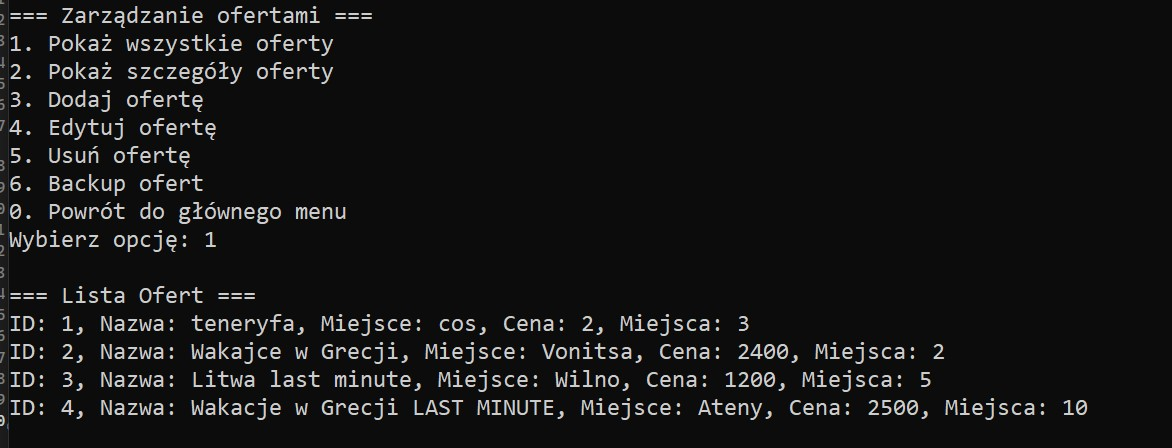
\includegraphics[width=0.9\textwidth]{figures/lista_ofert.jpg} 
  \caption{Zarządzanie ofertami}
  \label{fig:obrazek}
\end{figure}

\subsection{Moduł rezerwacji}
W podmenu rezerwacji użytkownik może:
\begin{itemize}
    \item \textbf{Dodać nową rezerwację} – wprowadzając identyfikator oferty, dane klienta i liczbę miejsc, co pozwala na rejestrację rezerwacji w systemie.
    \item \textbf{Edytować istniejącą rezerwację} – umożliwiając aktualizację danych rezerwacji (np. zmiana liczby miejsc lub korekta danych klienta).
    \item \textbf{Anulować rezerwację} – usuwając rezerwację, gdy zajdzie taka potrzeba.
    \item \textbf{Wyświetlić listę wszystkich rezerwacji} – co pozwala na bieżący przegląd dokonanych rezerwacji.
\end{itemize}
\newpage
\subsection{Moduł rezerwacji - dodawanie rezerwacji}
Poniżej przedstawiony sposób możliwości dodawania rezerwacji: 
\begin{figure}[htbp]
  \centering
  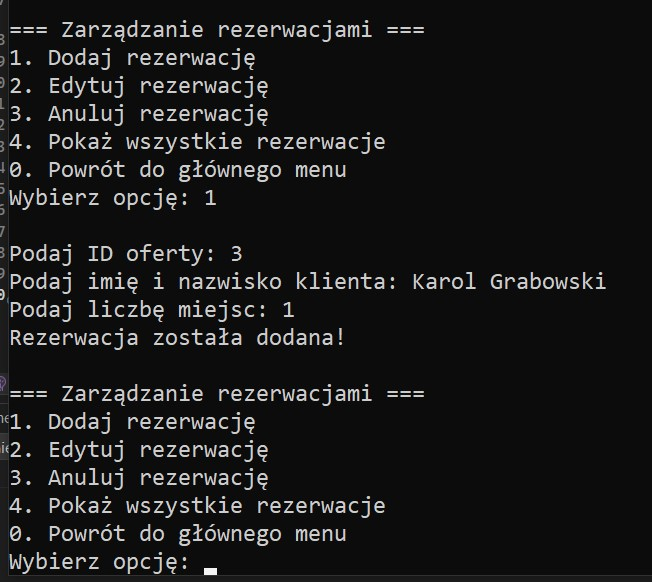
\includegraphics[width=0.9\textwidth]{figures/rezerwacja.jpg} 
  \caption{Zarządzanie rezerwacjami}
  \label{fig:obrazek}
\end{figure}


\subsection{Moduł Płatności}
Podmenu płatności umożliwia:
\begin{itemize}
    \item \textbf{Dodanie nowej płatności} – na podstawie identyfikatora rezerwacji, kwoty i daty płatności.
    \item \textbf{Wyświetlenie listy płatności} – system prezentuje wszystkie dokonane transakcje.
    \item \textbf{Generowanie faktur} – po podaniu ID płatności, system generuje sformatowaną fakturę, zawierającą kluczowe informacje o transakcji.
\end{itemize}


\subsection{Moduł Użytkowników}
\begin{itemize}
    \item \textbf{Dodawanie nowych użytkowników} – umożliwiając rejestrację nowych kont wraz z przypisaniem roli (administrator, pracownik, klient).
    \item \textbf{Edycja danych użytkowników} – co pozwala na aktualizację informacji takich jak nazwa czy przypisana rola.
    \item \textbf{Usuwanie użytkowników} – umożliwiając kontrolę nad dostępem do systemu.
    \item \textbf{Wyświetlanie listy użytkowników} – co pozwala na szybki przegląd dostępnych kont.
\end{itemize}

\section{Interakcja i Walidacja}
Interfejs konsolowy został zaprojektowany tak, aby zapewnić czytelne komunikaty oraz intuicyjne wprowadzanie danych. Każda operacja jest poprzedzona instrukcjami wyświetlanymi na ekranie, a system sprawdza poprawność wprowadzonych danych (np. weryfikacja, czy podana cena ma właściwy format lub czy liczba miejsc jest liczbą całkowitą). Dzięki temu użytkownik otrzymuje natychmiastową informację zwrotną o poprawności swojej operacji, co zmniejsza ryzyko błędów.


\subsection{Zalety Interfejsu Konsolowego}
Mimo że interfejs jest oparty na konsoli, ma on kilka istotnych zalet:
\begin{description}
    \item[Prostota:] System opiera się na przejrzystym menu, co pozwala na szybkie opanowanie obsługi aplikacji nawet przez osoby niezaznajomione z technologiami informatycznymi.
    \item[Łatwość Utrzymania:] Dzięki modularnej budowie menu oraz oddzieleniu logiki biznesowej, przyszłe modyfikacje lub rozbudowa interfejsu są łatwe do wykonania.
    \item[Szybkość Działania:] Aplikacja reaguje natychmiastowo na wprowadzane komendy, co zwiększa efektywność pracy użytkownika.
\end{description}

\section{Podsumowanie warstwy użytkowej}
Warstwa użytkowa systemu "Biuro Podróży" jest kluczowym elementem, który umożliwia użytkownikom efektywną interakcję z systemem. Dzięki dobrze zaprojektowanemu interfejsowi konsolowemu, użytkownicy mogą łatwo przechodzić między różnymi modułami systemu – od zarządzania ofertami, poprzez rezerwacje i płatności, aż po zarządzanie użytkownikami. Jasno zdefiniowane komunikaty oraz mechanizmy walidacji wprowadzanych danych zapewniają stabilność i przejrzystość działania systemu, co stanowi solidną podstawę do dalszej rozbudowy, na przykład o graficzny interfejs użytkownika lub dodatkowe mechanizmy zabezpieczeń.

\section{Poszczególne opcje programu}

\begin{figure}[htbp]
  \centering
  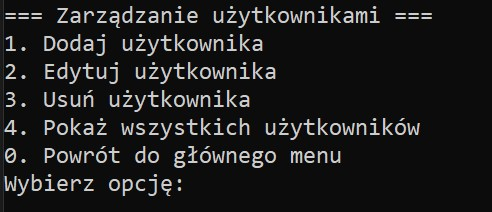
\includegraphics[width=0.9\textwidth]{figures/zarzadzanie_urzytkownikami.jpg} 
  \caption{Zarządzanie użytkownikami}
  \label{fig:obrazek}
\end{figure}

\begin{figure}[htbp]
  \centering
  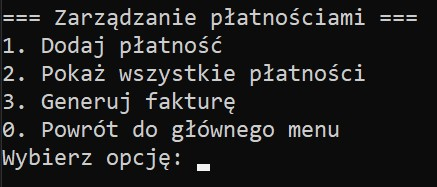
\includegraphics[width=0.9\textwidth]{figures/zarzadzanie_platnosciami.jpg} 
  \caption{Zarządzanie płatnościami}
  \label{fig:obrazek}
\end{figure}


% ********** Koniec rozdziału **********

\newpage
% ********** Rozdział 4 **********
\chapter{Podsumowanie}

Projekt systemu zarządzania biurem podróży, napisany w języku C\#, stanowi przykład rozwiązania informatycznego opartego na modularnej architekturze, w której kluczową rolę odgrywają trzy główne warstwy: modele danych, logika biznesowa oraz interfejs użytkownika. Modele danych, takie jak Oferta, Rezerwacja, Płatność oraz Użytkownik, służą do przechowywania podstawowych informacji niezbędnych dla funkcjonowania systemu. Dedykowane klasy zarządzające, odpowiadające za operacje CRUD oraz dodatkowe funkcjonalności, jak tworzenie kopii zapasowych, generowanie faktur czy kontrola dostępu, umożliwiają sprawną obsługę danych. Warstwa interfejsu, mimo że opiera się na konsolowym menu, zapewnia intuicyjną i przejrzystą interakcję, umożliwiając użytkownikowi łatwą nawigację między poszczególnymi modułami systemu.

Realizacja projektu wiązała się z wieloma wyzwaniami, z których najważniejsze dotyczyły stworzenia spójnej architektury systemu oraz zapewnienia integralności danych przechowywanych w formacie JSON. Przypisywanie unikalnych identyfikatorów oraz wdrożenie mechanizmu tworzenia kopii zapasowych wymagało precyzyjnego podejścia i iteracyjnego testowania. Dodatkowo, walidacja danych wprowadzanych przez użytkowników oraz projektowanie czytelnego interfejsu konsolowego stanowiły istotne aspekty, których celem było zminimalizowanie błędów i zapewnienie stabilności działania systemu.

Podsumowując, projekt umożliwia skuteczne zarządzanie ofertami turystycznymi, rezerwacjami oraz rozliczeniami finansowymi, stanowiąc solidną bazę do dalszych rozwoju. W przyszłości system można udoskonalić poprzez migrację danych do dedykowanej bazy, integrację z zewnętrznymi platformami płatności, wdrożenie graficznego interfejsu użytkownika oraz implementację zaawansowanych mechanizmów bezpieczeństwa, takich jak dwuskładnikowe uwierzytelnianie i szyfrowanie danych. Takie usprawnienia pozwolą na obsługę większych obciążeń oraz podniosą poziom ochrony informacji, co wpłynie na zwiększenie efektywności i atrakcyjności systemu na rynku.


% ********** Koniec rozdziału **********


\newpage
\input{R6.tex}
\newpage

% *************** Bibliografia ***************
\begin{thebibliography}{6}
\addcontentsline{toc}{chapter}{Bibliografia}
%dodanie wpisu do spisu bibliograficznego
\bibitem{Sommerville2015} Sommerville, I. (2015). \textit{Inżynieria oprogramowania}. Wydawnictwo Helion.

\bibitem{Martin2009} Martin, R. C. (2009). \textit{Czysty kod. Podręcznik dobrego programisty}. Wydawnictwo Helion.

\bibitem{Sutherland2014} Sutherland, J. (2014). \textit{Scrum. Zwinne zarządzanie projektami}. Wydawnictwo Helion.

\bibitem{MSGuide} Microsoft. (n.d.). \textit{C\# Programming Guide}. Dostępne pod adresem: \url{https://docs.microsoft.com/pl-pl/dotnet/csharp/}.

\bibitem{MSJson} Microsoft. (n.d.). \textit{System.Text.Json Namespace}. Dostępne pod adresem: \url{https://docs.microsoft.com/pl-pl/dotnet/api/system.text.json}.

\bibitem{JSONorg} JSON.org. (n.d.). \textit{JSON: The JavaScript Object Notation}. Dostępne pod adresem: \url{https://www.json.org/json-en.html}.

\bibitem{AgileManifesto} Agile Manifesto. (2001). \textit{Manifesto for Agile Software Development}. Dostępne pod adresem: \url{https://agilemanifesto.org}.

\end{thebibliography}
\newpage

% *************** Zakończenie ***************
% *************** Zakończenie ***************

%***************************************************************************************
% W tym miejscu znajdują się polecenia odpowiedzialne za tworzenie
% spisu ilustracji, spisu treści oraz streszczenia pracy
%***************************************************************************************

%spis rysunków
\addcontentsline{toc}{chapter}{Spis rysunków}
\listoffigures
\newpage

%spis tablic
\addcontentsline{toc}{chapter}{Spis tablic}
\listoftables
\newpage

% %streszczenie
% \addcontentsline{toc}{chapter}{Streszczenie}
% \noindent
% {\footnotesize{}\textbf{Wyższa Szkoła Informatyki i Zarządzania z siedzibą w Rzeszowie\\
% Kolegium Informatyki Stosowanej}
% \vspace{30pt}

% \begin{center}
% \textbf{Streszczenie pracy dyplomowej inżynierskiej}\\
% \temat
% \end{center}

% \vspace{30pt}
% \noindent
% \textbf{Autor: \autor
% \\Promotor: \promotor
% \\Słowa kluczowe: tutaj umieść słowa kluczowe}
% \vspace{40pt}
% \\Treść streszczenia, czyli kilka zdań dotyczących treści pracy dyplomowej w języku polskim.
% \vspace{80pt}

% \noindent
% \textbf{The University of Information Technology and Management in Rzeszow\\
% Faculty of Applied Information Technology}
% \vspace{30pt}

% \begin{center}
% \textbf{Thesis Summary\\}
% Tytuł pracy w języku angielskim
% \end{center}

% \vspace{30pt}
% \noindent
% \textbf{Author: \autor
% \\Supervisor: \promotor
% \\Key words: tutaj umieść słowa kluczowe}
% \vspace{40pt}
% \\Treść streszczenia, czyli kilka zdań dotyczących treści pracy dyplomowej w języku angielskim - tłumaczenie tekstu z języka polskiego.
% }

% *************** Koniec pliku back.tex ***************


\end{document}
% *************** Koniec pliku szablon.tex ***************
